\documentclass[11pt]{article}

\usepackage{natbib}
\usepackage{appendix}
\usepackage{hyperref}
\hypersetup{hidelinks,
	colorlinks=true,
	allcolors=black,
	pdfstartview=Fit,
	breaklinks=true}
\usepackage{booktabs}
\usepackage{graphicx}
\usepackage{float}
\usepackage{texcount}

\begin{titlepage} 
  \center 
  

  \textsc{\LARGE MSc Computational Methods in Ecology and Evolution}\\[1.5cm] % Name of your university/college
  \textsc{\Large Imperial College London}\\[0.5cm] % Major heading such as course name
  \textsc{\large Department of Life Science}\\[0.5cm] % Minor heading such as course title
 
  \makeatletter
  \HRule \\[0.8cm]
  {\bfseries \@title}\\[0.8cm] Non-linear least squares Gompertz models outperform linear models and non-linear Logistic growth models in fitting microbial population growth date
  \HRule \\[1.5cm]
   
  
  
  \begin{minipage}{0.5\textwidth}
  \begin{flushleft} \large
  \emph{Author:}\\
  \@author Chuxinyao Wang
  \end{flushleft}
  \end{minipage}\\
  
  ~
  \begin{minipage}{0.5\textwidth}
  \begin{flushright} \large
  \emph{Word count:} \\
  2025 \\[1.2em] % Supervisor's Name
  \end{flushright}
  \end{minipage}\\[2cm]
  \makeatother
  

  
{\large \today}\\[2cm] % Date, change the \today to a set date if you want to be precise
  
  \vfill % Fill the rest of the page with whitespace
  
  \end{titlepage}
\title{Non-linear least squares Gompertz models outperform linear models and non-linear Logistic growth models in fitting microbial population growth data}

\author{Chuxinyao Wang}

\date{November 2022}
\newpage
\begin{document}
\maketitle
  
\begin{abstract}
AIC has been widely used in ecology, particularly in relation to model selection and model ranking.
In this paper, 285 sets of microbial growth data were input and models were fitted to those data sets by using computational methods with R. 
The data were fitted by using a total of 6 models in both types of linear and non-linear least squared fits. 
By comparing the $AIC$, $AIC_c$ and adjusted $R^2$ values of each model with the 285 data sets, the logistic growth model model was found to be stable for the majority of the 285 data sets and was the final optimal model option.
\end{abstract}
  
\section{Introduction}
Microbiology has long used growth rates to quantify phenotypic properties to determine bacterial growth rates, and growth rates are an important basis for all areas of microbiology \citep{10.1093/molbev/mst187}. And the rate of change affects the trend of population growth. Estimating population growth has become a central focus of population biology. The use of modeling to fit population growth trends can more generally represent the population changes of a species. Much ecological work needs to drive the development of new predictive ecological methods that can reliably predict future changes in population size \citep{matthiopoulos2019predicting}. Therefore, modelling population growth came into being. The purpose of this article is to evaluate and select the model, and the standard used is to compare and compare $AIC$, $AIC_{c}$, and adjusted $R^{2}$ values based on procedures written by \cite{johnson2004model} .The Akaike Information Criterion ($AIC$) is an important reference index in the comparison of models in the field of ecology, where it is often necessary to compare and rank a number of potentially available models and to assess which of them is better able to deliver the expected results in the biological processes under study \citep{Symonds2010ABG}. And, \cite{STEPHENS2007192} also mention the tendency of using IT techniques such as $AIC$ to replace null hypothesis significance testings in ecology, although many ecologists are still opposed to such IT techniques as model selection under ecological applications, arguing that they do not facilitate the development of hypothesis sets \citep{10.2307/3802765, ctx43114213010001591}.\\

Regardless of whether the influence of IT technology on statistics is controversial or not, this paper mainly uses this feasible IT technology method to evaluate the proposed possible population growth model, and uses $AIC$ as a criterion for assessing the fit of the model to compare the goodness of the models then select the best model among competing models.


\section{Methods}

\subsection{Data collection}
The data used to evaluate the model this time came from data on the growth of various microbial populations sampled in different journals(\href{https://github.com/mhasoba/TheMulQuaBio/blob/master/content/data/LogisticGrowthData.csv}{Data address}). A total of 285 sets of data were obtained after classification by computer methods. The 285 sets of data include differences such as different species, different temperatures, and different culture media (see metadata in the Appendix. 1 for details), which makes model selections more convincing and allows them to be verified under different conditions.

\subsection{Candidate Models}
As mentioned by \cite{johnson2004model}, articulating a reasonable set of competing models should be chosen prior to data collection. The data was provided for model selection without my intervention, so the proposal of the candidate models can be regarded as the proposal before knowing the data. Considering the rationality and diversity of the model, the model is selected from the linear model and the nonlinear model respectively. The first is the linear function model:
\begin{equation}
    {N}={r}\cdot{t}+{N_0}
\end{equation}

Considering that population growth is affected by the growth rate and the initial population, the linear function of the growth rate as the slope and the initial population as the intercept is used as the first candidate model.
The second model considers that the linear relationship of population growth may have a linear relationship between the logarithm of the population and time, so the second model is also a linear function model, but the dependent variable is changed to the logarithm of the population, and the intercept is also changed to Logarithm of the initial population size:
\begin{equation}
    {logN}={r}\cdot{t}+{logN_0}
\end{equation}
\\
The third model considers that in addition to the growth rate, there are some unknown factors ($a_1$ and $a_2$ in $Equation_(3)$) that have an impact on the population change, so the quadratic polynomial linear model is used as the third alternative model:
\begin{equation}
    {N}={a_1}\cdot{t^2}+{a_2}\cdot{t}+{N_0}
\end{equation}
\\
Similarly, the logarithm of the population may have a linear relationship with the influencing factors($b_1$ and $b_2$ in $Equation_(4)$), so the logarithm of the population is used as a quadratic polynomial model as the fourth alternative model:
\begin{equation}
    {logN}={b_1}\cdot{t^2}+{b_2}\cdot{t}+{logN_0}
\end{equation}
\\
The fifth model takes nonlinear model and logistic model as alternative models. It is an important equation of population biology, proposed by Verhulst in 1938 \citep{verhulst1838notice}. This model also takes into account the capacity of the environment, that is, the maximum number of people in a limited environment. The reason for including this model in the alternative model is also to determine the reliability of this model among many models. The differential equation form of the logistic growth model is expressed as:
\begin{equation}
    \frac{dN}{dt} = r\cdot N\cdot (1 - \frac{N}{K})
\end{equation}
\\
For the sixth model, I used the Gompertz model, a commonly used model for microbial population growth \citep{doi:10.1128/aem.56.6.1875-1881.1990}. According to \cite{BUCHANAN1997313}, the characteristic of this model is that the bacterial growth curve is divided into three phases: lag, stationary and exponential according to different growth rates. The model has four parameters: $\log N_{0}$ ($\log$ of initial population), $\log N_{MAX}$ ($\log$ of maximum population) , $t_{lag}$ (time when the lag phase ends), and $t_{MAX}$ (time when the exponential phase ends). Gompertz model equation is:
\begin{equation}
    \log_{N_t}=N_{0}+(N_{MAX}-N_{0})\cdot e^{-e\cdot r_{max}\cdot exp(1)\frac{t_{lag}-{t}}{(N_{MAX}-N_{0})\cdot \log_{10}+1}}
\end{equation}
\\
These six models were all imported into the computer, tested one by one using the above 285 sets of data, and fitted the data into the model.

\subsection{Model Fitting and Comparison}
The process of model fitting requires the use of a computer. In R, after the six models are written, a preliminary test of the model is required. After grouping the original data, substituting a group of data to conduct preliminary verification on whether the model is reasonable, and the verification model can better reflect the changing trend of the data.\\

After completing the preliminary model and rationality verification, 285 sets of data need to be imported circularly, and the model comparison criteria, ie. $AIC$ $AIC_c$, and adjusted $R^2$, are performed through the computer, and each set of calculated data is stored in turn for consequent comparison. For the calculation of $AIC$ and $AIC_c$, I set the calculation scale on the exponential scale. Since all the models on the logarithmic scale, the dependent variables are often negative and unable to be calculated in the $AIC$ calculation (involving the second order Logarithmic operation), so models under scale of logarithm were taken the natural logarithm index $e$ of the dependent variable before calculating the sum of squared residuals, and then perform scale matching with other non-logarithmic scale models, thus $AIC$, $AICc$ comparison are more precise.\\

In addition, the reason why $AIC$ and $AIC_c$ are used as comparison criterion both is that in the 285 sets of data, the number of each set of data is different, while $AIC_c$ is more accurate when the amount of data is small, and when the amount of data is large to a certain extent, the calculation result of $AIC_c$ is basically $AIC$ \citep{brewer2016relative}. Therefore, including the two criteria at the same time for comparison can double judge the performance of the model under the same set of data.\\

For the final model comparison link, how to deal with the obtained $AIC$, $AIC_c$ and adjusted $R^2$ becomes the focus of comparison. In \cite{johnson2004model} Model selecting approach part, they performed the likelihood calculation on $AIC$ and compared the weight assignment of each model. This is a relatively complete and complicated process. I simplified it to make it easier to understand and accept. Specifically, the distribution of $AIC$ and $AIC_c$ is visualized and analyzed first. And calculate the average and variance of $AIC$ and $AIC_c$ of each model, and compare $AIC_c$ first. In general, the smaller the average of $AIC_c$ and $AIC$, the better the model. If the average of the models is not much different Next, compare its stability, that is, variance comparison. The adjusted $R^2$ is finally used as an auxiliary comparison index, and the closer to 1, the better model is.

\subsection{Computing languages and tools}
The computer language used in the whole process of model selection analysis and the use of each package will be presented in the following table.

\begin{table*}[htbp]
    \centering
    \caption{Computing languages and tools use}
    \label{tab:univ-compa}
    \begin{tabular}{lcl}
    \toprule
         \textbf{Computer languages} & \textbf{Packages} & \textbf{Uses}\\ \midrule
         \textbf{Python} & Pandas & Data grouping and storing\\
         \midrule
         \textbf{R} & ggplot2 & Preliminary model fitting inspe- \\
         &  & ction work and model comparison\\
         & & criteria distribution  plot drawing\\
          &  minpack.lm & Fit nonlinear Models using the  \\
         &  & Levenberg-Marquardt Algorithm\\
         & & within the package\\
        & ggpubr & Typesetting for diagrams\\
        \midrule
       \textbf{LaTeX} & natbib & Set the Citation and reference \\
        & & format to Harvard\\
        & appendix & Create appendix\\
         & hyperref & Create a link to direct \\
        & & to the data source address\\
        & booktabs & Create tables\\
        & graphicx & Input figures  \\
        \midrule
        \textbf{Bash} & & Compile Miniproject report \\
        \toprule
    \end{tabular}
    \label{tab:my_label}
\end{table*}

\newpage
\section{Results}
The calculation results of $AIC$, $AIC_c$, and adjusted $R^2$ descriptive statistics of each model are shown in Table 2, 3, and 4. From the mean and median of the $AIC$ values, the $AIC$ value of the Gompertz model is significantly smaller than that of the other 5 models' $AIC$. Also, $AIC_c$ values have the same result, Gompertz also has the smallest $AIC_c$ value. \\

\begin{table}[H]
\centering
\caption{Descriptive statistics for $AIC$}
\begin{tabular}{llllll}
\toprule
& \textbf{model type} & \textbf{mean}& \textbf{median} & \textbf{min} & \textbf{max} \\ \toprule
 & linear model & 133.02 & 96.24 & -265.78 & 2423.012 \\
 & log linear model & 162.73  & 105.82 & -262.19 & 3038.23 \\
 & polynomial model & 118.43 & 87.46 & -267.74 & 2419.19 \\
 & log polynomial model & 133.65  & 94.42 & -265.31 & 2467.60 \\
 & logistic model & 83.49 & 67.23 & -253.09 & 1917.48 \\
 & gompertz model & 5.68 & 12.78 & -319.09 & 16.24 \\ 
 \bottomrule
\end{tabular}
\end{table}

\begin{table}[H]
\centering
\caption{Descriptive statistics for $AIC_c$}
\begin{tabular}{llllll}
\toprule
 & \textbf{model type} & \textbf{mean}& \textbf{median} & \textbf{min} & \textbf{max}              \\ \toprule
 & linear model         & 137.86 & 105.00 & -264.74 & 2423.18 \\
 & log linear mdoel     & 156.73  & 99.82 & -268.19 & 3032.23 \\
 & polynomial model     & 127.68 & 108.16 & -265.92 & 2419.47 \\
 & log polynomial model & 142.90  & 112.78 & -263.49 & 2467.88 \\
 & logistic model       & 90.74 & 81.59 & -251.35 & 1917.86 \\
 & gompertz model       & 13.01 & 17.23 & -318.82 & 36.24\\
\bottomrule
\end{tabular}
\end{table}

\begin{table}[H]
\centering
\caption{Descriptive statistics for Adjusted $R^2$}
\begin{tabular}{llllll}
\toprule
 & \textbf{model type} & \textbf{mean}& \textbf{median} & \textbf{min} & \textbf{max}              \\ \toprule
 & linear model         & -1768.3980 & 0.3870 & -466006.9655 & 0.9826 \\
 & log linear mdoel     & -10.9571  & 0.6247 & -1133.3364 & 0.9931 \\
 & polynomial model     & 0.3590 & 0.8125 & -23.2333 & 1.1204 \\
 & log polynomial model & 0.4334  & 0.8655 & -23.1136 & 1.1157 \\
 & logistic model       & -3.5253e+28 & 0.9492 & -7.6852e+30 & 0.99996 \\
 & gompertz model       & 0.1168 & 0.9779 & -23.8145 & 0.9988\\
\bottomrule
\end{tabular}
\end{table}

However, in the adjusted $R^2$ table, large outliers appear, which is reflected in the large deviation of the adjusted $R^2$ values of the six models from the median. The minimum adjusted $R^2$ value of each group of models is far less than 1. Even in the logistic model, the adjusted $R^2$ value fitted by one data is too small to be regarded as an invalid value. Therefore, it is more efficient to compare medians here. From Table 3, the Gompertz model wins again among the six models, the median of adjusted $R^2$ is closest to 1.\\

The distribution box plots of $AIC$, $AIC_c$, and adjusted $R^2$ in the six models are shown in Figures 1, 2, and 3.\\

\begin{figure}[htbp]  
\centering
\rotatebox{270}{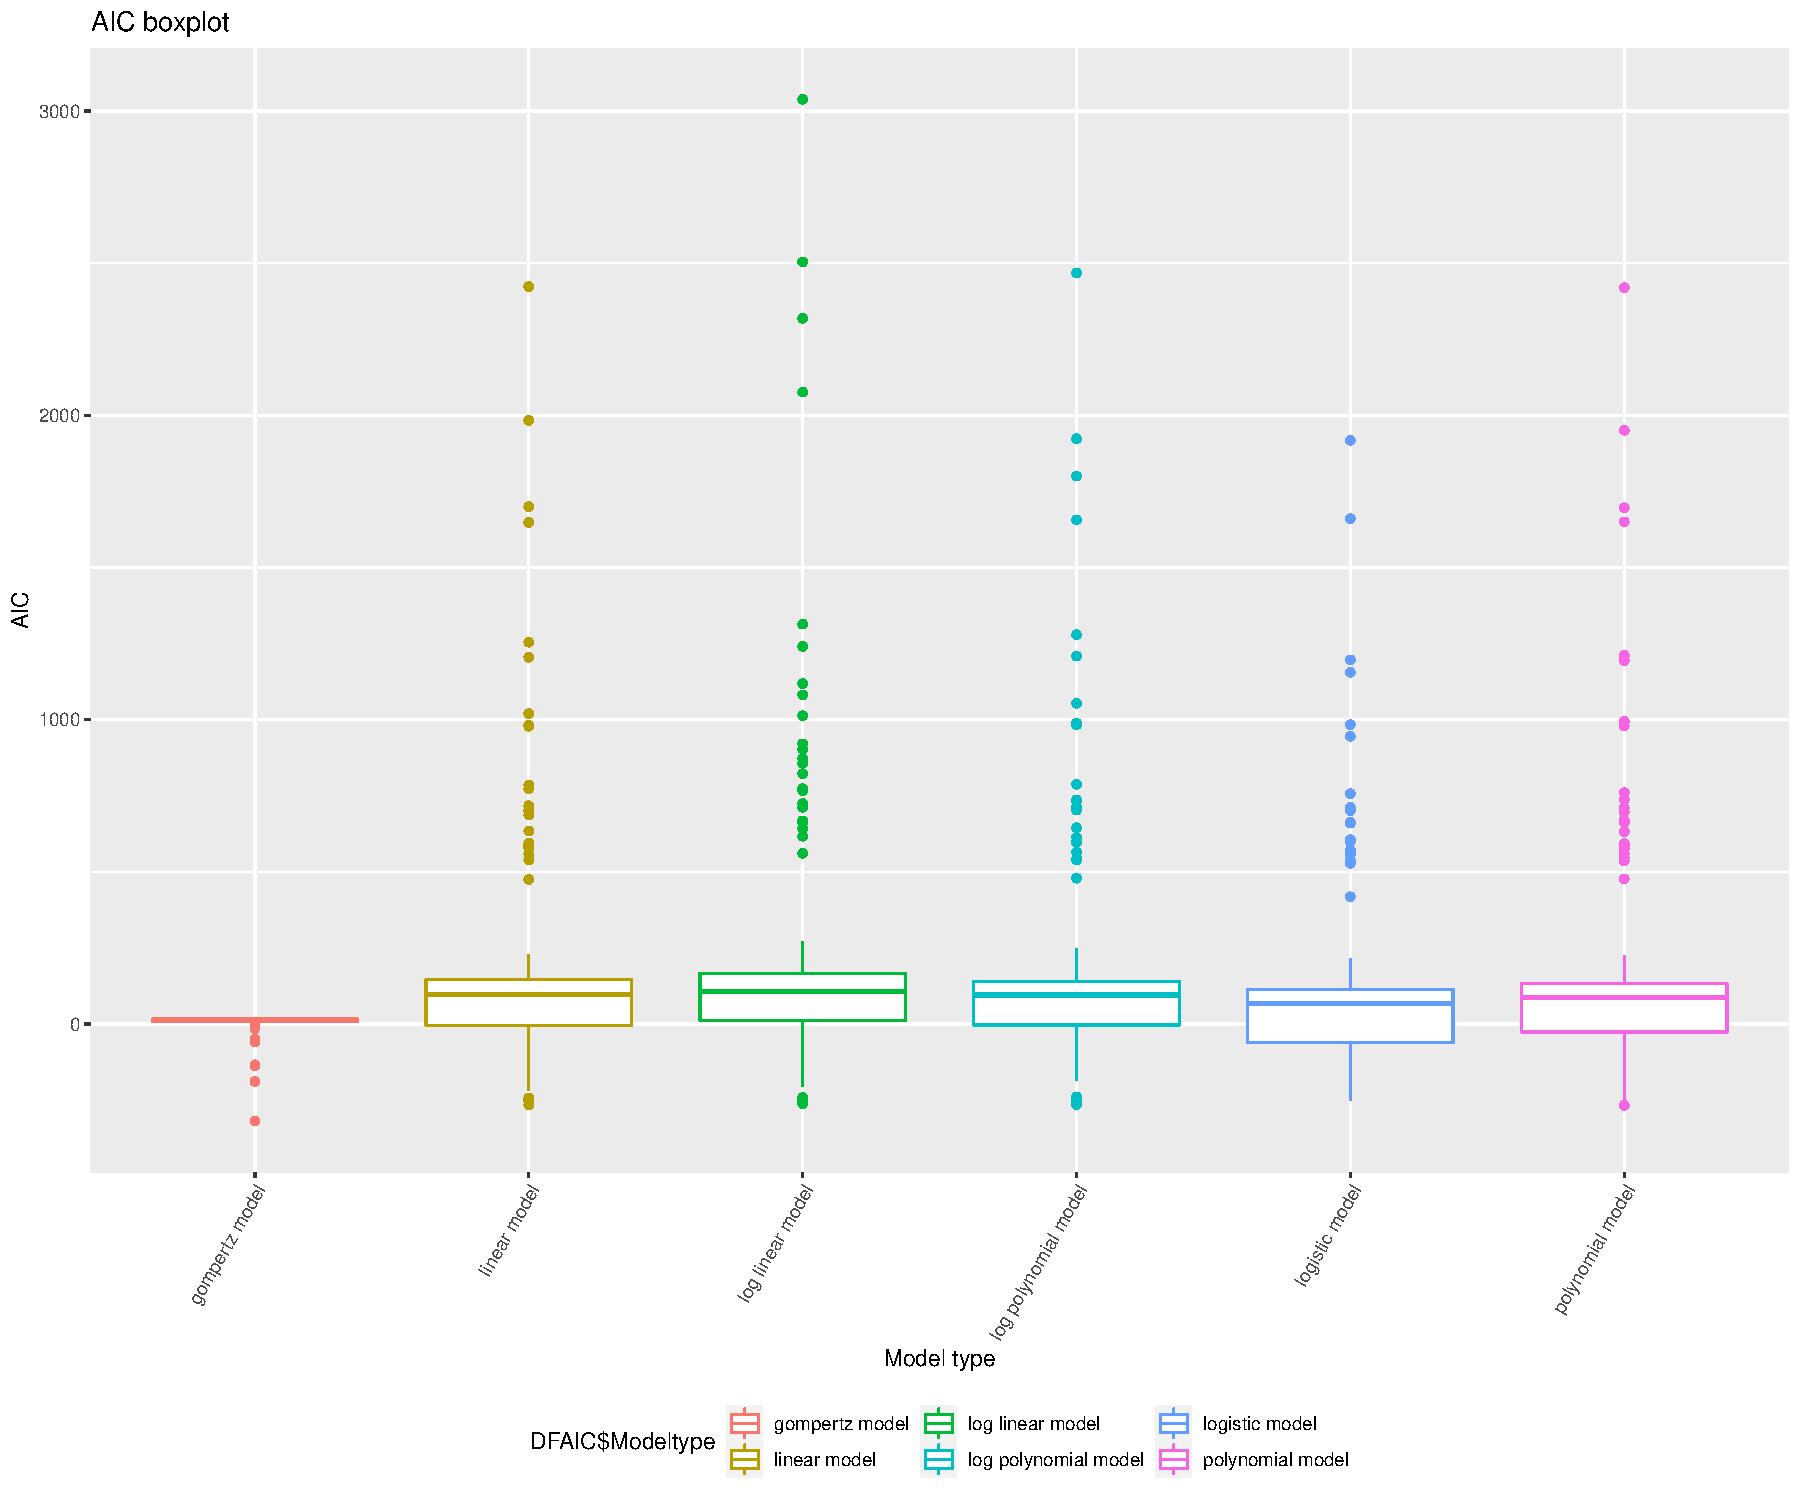
\includegraphics[height=15cm,width=18cm]{aic.pdf}}
\caption{Box plot of $AIC$}
\end{figure}

\begin{figure}[htbp]
\centering
\rotatebox{270}{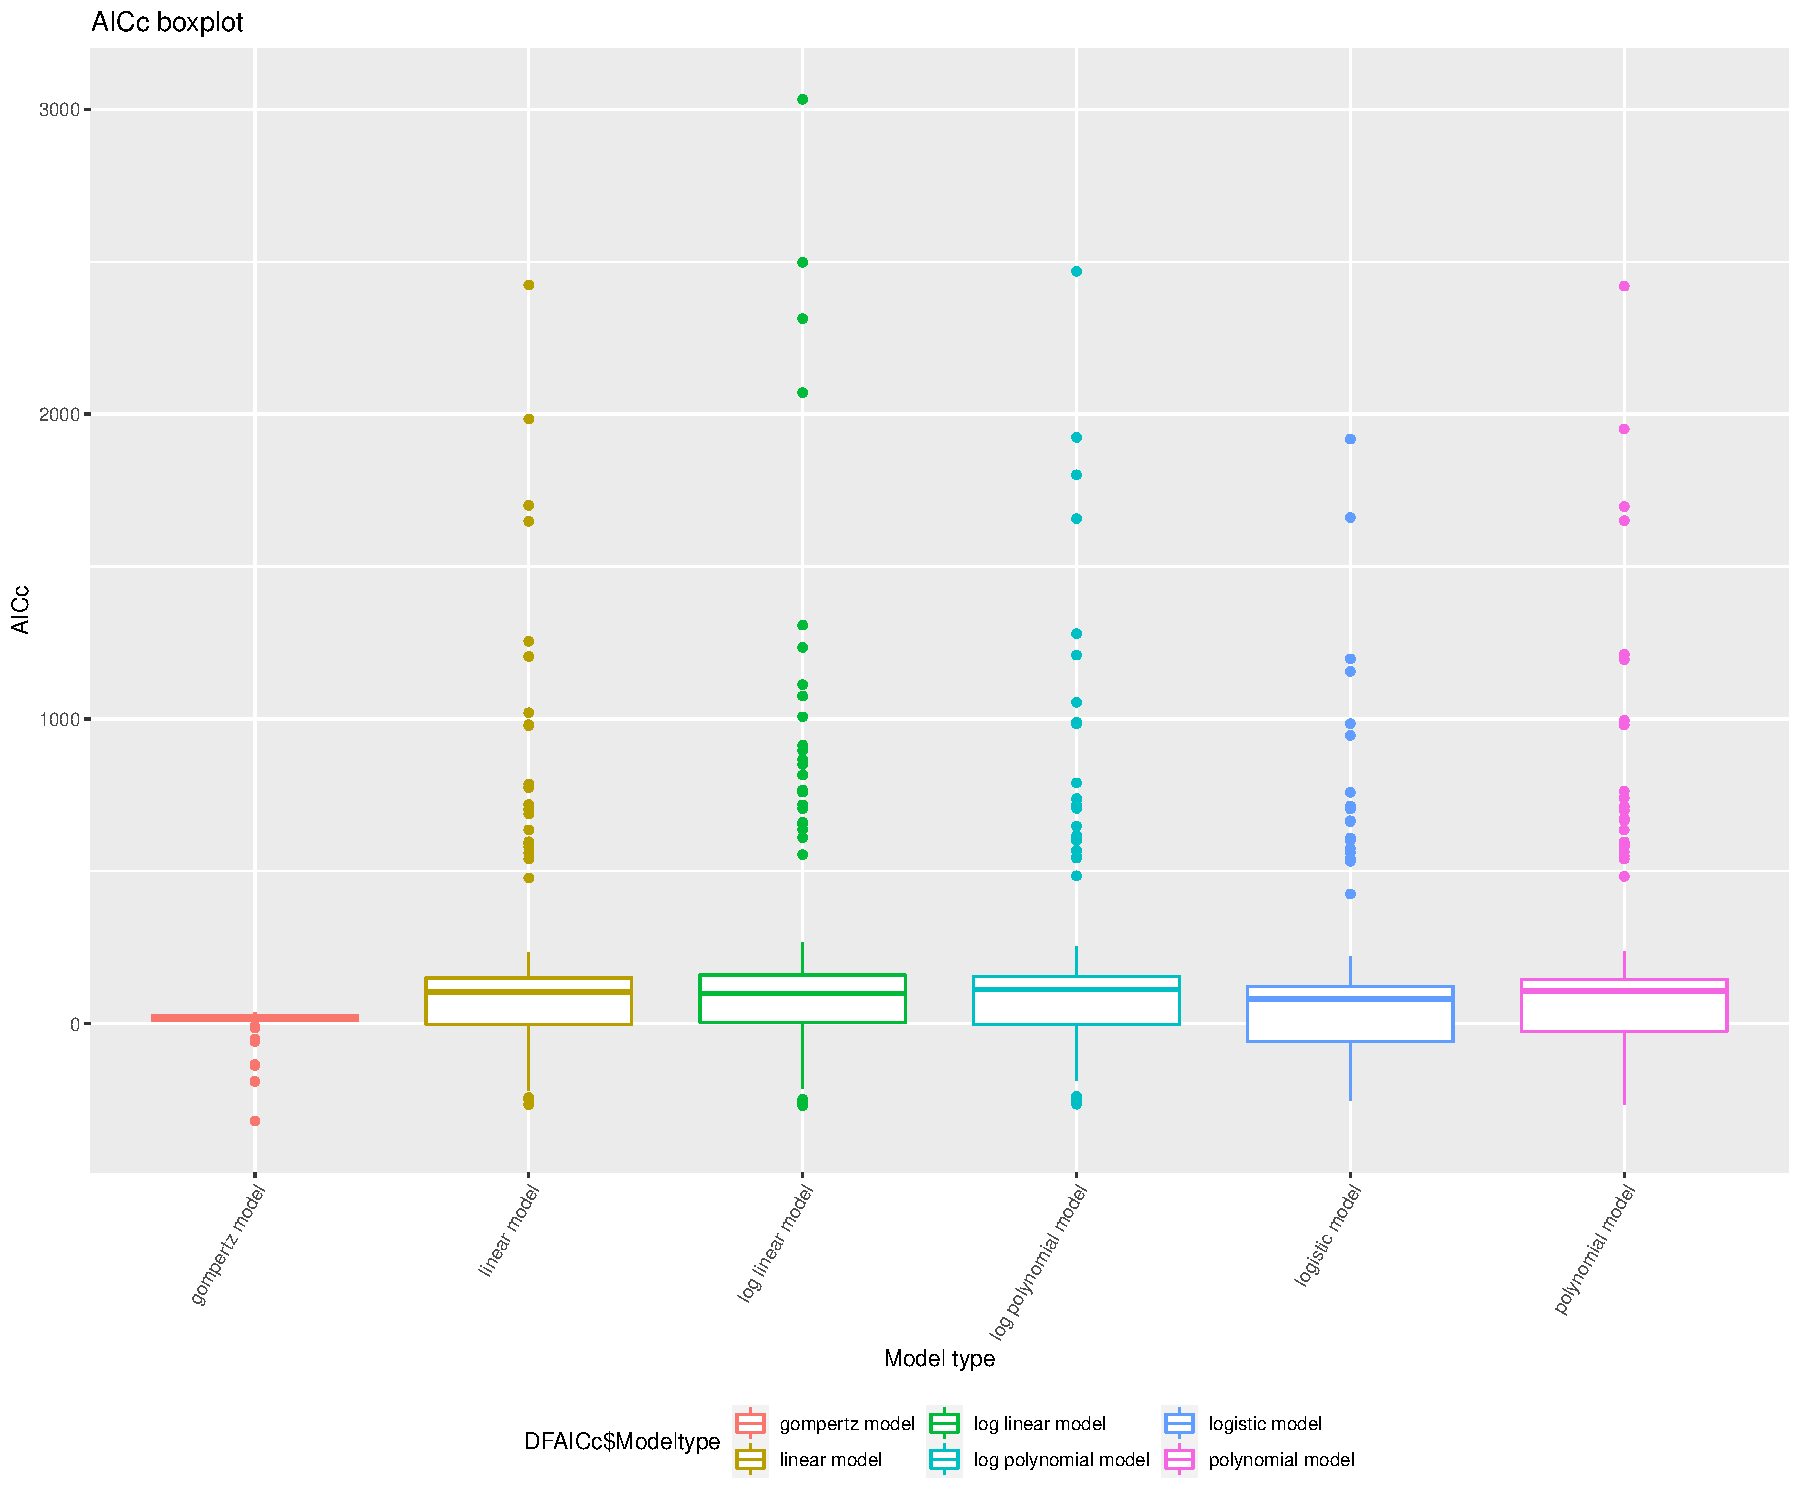
\includegraphics[height=15cm,width=18cm]{aicc.pdf}}
\caption{Box plot of $AIC_c$}
\end{figure}

\begin{figure}[htbp]
\centering
\rotatebox{270}{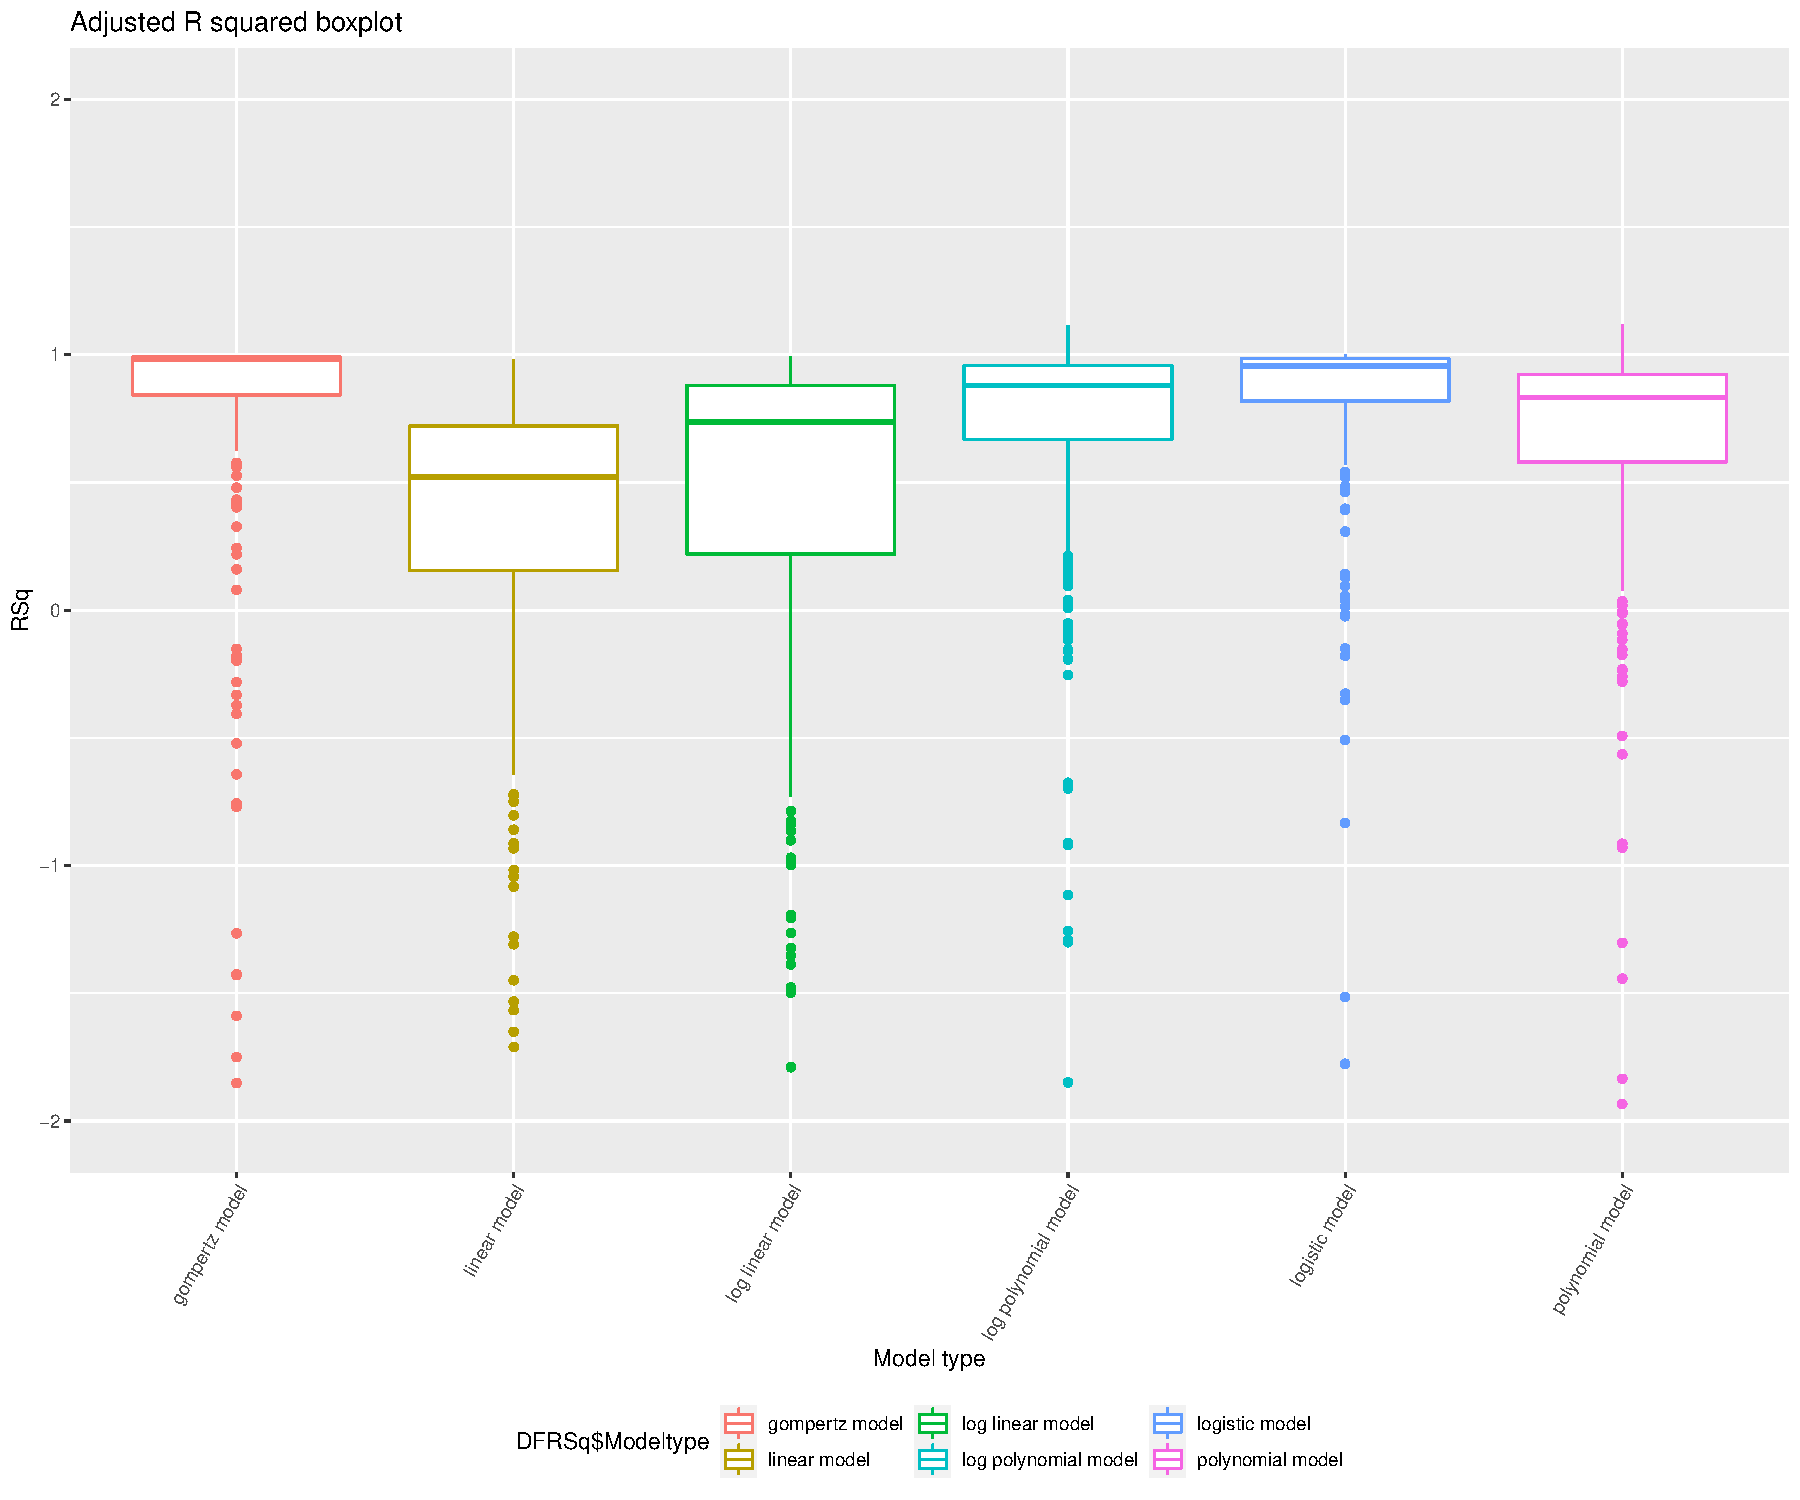
\includegraphics[height=15cm,width=18cm]{rsq.pdf}}
\caption{Box plot of adjusted $R^2$}
\end{figure} 

In the box plots of the first two $AIC$ and $AIC_c$ values, the Gompertz model is very stable, with fewer outliers than the other five groups of models. The worse performance is the logarithmic linear model.\\

The adjusted $R^2$ box plot excludes outliers that are too small, so as to better present the distribution of the adjusted $R^2$ value of the data sample. In the adjusted $R^2$ box plot, it can be seen that the fit of the Gompertz and Logistic models to the data is better than that of several other models, while the fit of the linear model is the lowest overall.

\section{Discussion}
The aim of this paper is to rank how well the candidate models fit the data. By comparing the $AIC$, $AIC_c$, and adjusted $R^2$ of different data, it can be concluded that the $AIC$ and $AIC_c$ median of the Gompertz model are the lowest, and the Gompertz model has the most stable fitting results for all data, and has the highest adjusted R2 value . Therefore, it can basically be determined that the optimal model choice among the candidate population growth models is the Gompertz model. Secondly, except for the huge outliers in the adjusted $R^2$ value of the logistic model, its $AIC$ and $AIC_c$ are only larger than the Gompertz model, so the logistic model ranks second only to the Gompertz model. After a similar comparison, it can be determined that the final ranking is $1.Gompertz >2.Logistic> 3.Polynomial> 4. linear> 5.log polynomial> 6.log linear$. \\

It is important to note that the model with the logarithm is not as effective at fitting the data as the model without the logarithm. It appears that there is a weaker correlation between the population's logarithm and the influencing variables than there is between the population as a whole and the influencing factors, but Gompertz model just becomes the exception, performs the best and merits additional study because it is fitted on a logarithmic scale. \\

Besides, according to the $AIC$ value mentioned by \cite{brewer2016relative}, there is a penalty mechanism for the number of parameters, that is, the more parameters, the values of $AIC$ and $AIC_c$ will be reduced accordingly, and the same is true for the adjusted R2.(The number of parameters is $k_{linear}=3, k_{loglinear}=3, k_{polynomial}=4, k_{logpolynomial}=4, k_{logistic}=4, k_{gompertz}=4$) Therefore, $AIC$, $AIC_c$ and adjusted $R^2$ are compared between models with the same number of parameters Finally, the conclusions that can be drawn are consistent with the overall comparison and the rankings have not changed.\\

This model comparison study did not carry out deeper calculations such as \cite{johnson2004model} use of likelihood values and weighting scores to compare the fit between models, which was rougher and less accurate for model comparison and ranking. \\

Secondly, the data this time belong to the growth data of microbial population, lacking the comparison of the model fit to the change of population of other organisms. Perhaps, the best model in the growth of microbial population is Gompertz, but in a larger environment it may be The Gompertz model cannot better reflect the significant impact of the actual environment or other recessive factors on the biological population from a mathematical point of view. Therefore, considering the diversity of data is also a further determination of the performance of the model. Secondly, there are differences in data in different living environments (such as temperature, culture medium), which can also be used as one of the conditions to analyse the fitting status of the same set of candidate models under different environmental conditions, where research has been insufficient.

\newpage
\section{Appendix}

\begin{table}[H]
\caption{Meta data for 285 sets of data in model fitting}
\begin{tabular}{@{}ll@{}}

\toprule
Time          & Time at which measurement was taken.                          \\ \midrule
PopBio        & Population or biomass measurement.                            \\
Temp          & Temperature at which the microbe was grown (degrees Celsius). \\
Time units   & Units time is measured in.                                    \\
PopBio units & Units population or biomass are measured in.                  \\
Species       & Species or strain used.                                       \\
Medium        & Medium the microbe was grown in.                              \\
Rep           & Replicate within the experiment.                              \\
Citation      & Citation for the paper in which the study was recorded.       \\ \bottomrule
\end{tabular}
\end{table}



















\newpage
\bibliographystyle{agsm}

\bibliography{reference}

\end{document}
